% ============================================================
%  title_ru.tex — title page, Russian-language builds
%
%  Language-specific by design: no \iftoggle/\KZ/\RU branching
%  needed here, since a separate title_kz.tex (and, if the
%  bilingual experiment-tour title ever needs one, title_both.tex)
%  handles the other languages.
%
%  Required \OlympStringFallback slots (defined by build.py from
%  competitions.yaml / manifest.yaml, or manually below for
%  local testing):
%    name        — short competition name   (name.short.ru)
%    name_full   — full competition name     (name.full.ru)
%    stage       — competition stage         (name.stage.ru)
%    eventdates  — full event date range + city, precomputed
%                  by build.py from manifest.yaml's dates block
%
%  \OlympGrade is provided directly by olympiad.cls — no slot
%  needed for the grade number itself.
%
%  Tour icon is picked via the class's own \ifOlympTheory /
%  \ifOlympExperiment, not a legacy toggle.
% ============================================================

\thispagestyle{empty}

\vspace*{\fill}

\begin{center}
  \ifOlympTheory
    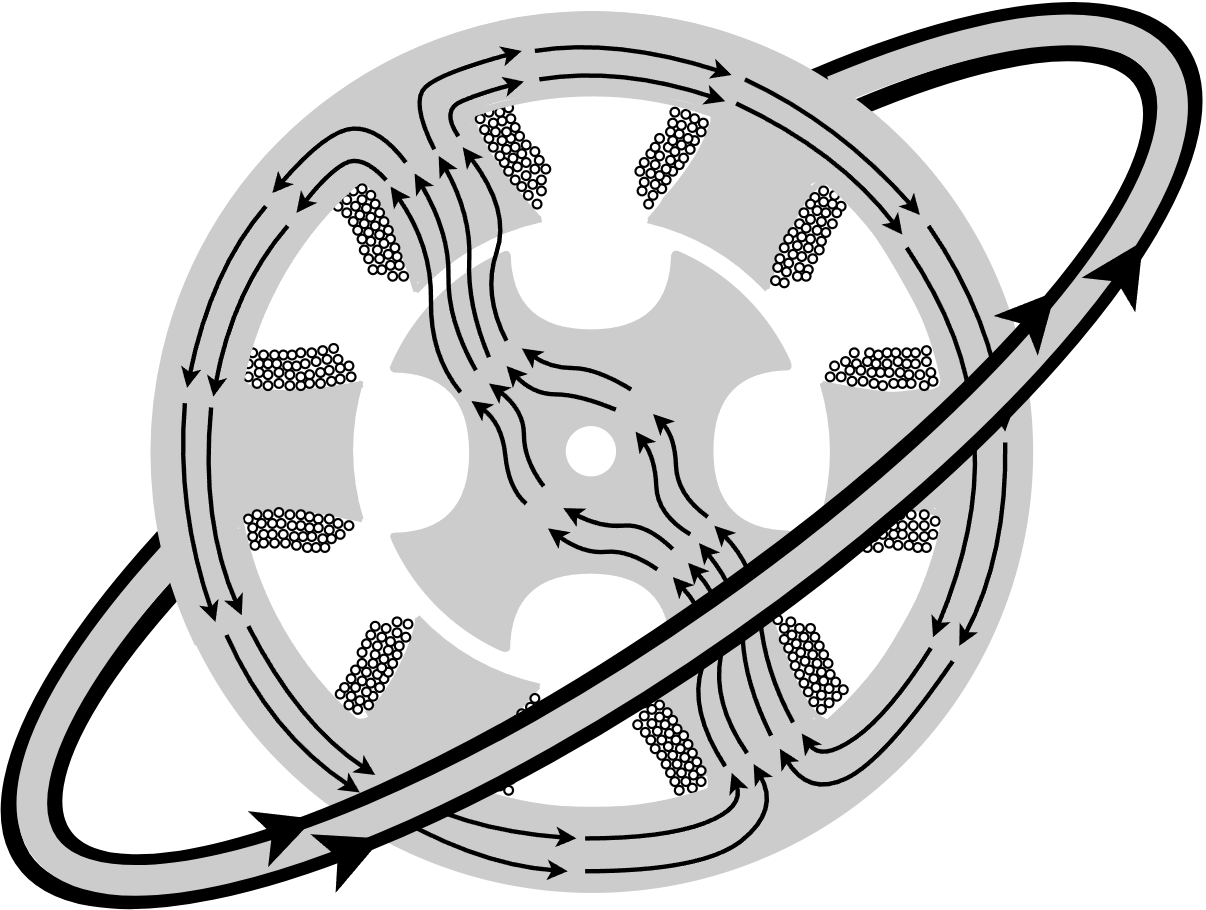
\includegraphics[width=0.6\linewidth]{../competitions/2025-26/respa/icon_theor.png}
  \fi
  \ifOlympExperiment
    
\includegraphics[width=0.6\linewidth]{../competitions/2025-26/respa/icon_exp.png}
  \fi
\end{center}

\vspace*{\fill}


\href{https://daryn.kz/respa/}{%
  
\includegraphics[width=0.2\linewidth]{daryn_logo.png}%
}

\textbf{\OlympStringFallback{name_full}}

\textit{\OlympStringFallback{stage}}

\textit{\OlympStringFallback{eventdates}}

\textit{Официальный комплект заданий \OlympGrade{} класса}

\newpage